% Options for packages loaded elsewhere
\PassOptionsToPackage{unicode}{hyperref}
\PassOptionsToPackage{hyphens}{url}
%
\documentclass[
]{article}
\usepackage{lmodern}
\usepackage{amssymb,amsmath}
\usepackage{ifxetex,ifluatex}
\ifnum 0\ifxetex 1\fi\ifluatex 1\fi=0 % if pdftex
  \usepackage[T1]{fontenc}
  \usepackage[utf8]{inputenc}
  \usepackage{textcomp} % provide euro and other symbols
\else % if luatex or xetex
  \usepackage{unicode-math}
  \defaultfontfeatures{Scale=MatchLowercase}
  \defaultfontfeatures[\rmfamily]{Ligatures=TeX,Scale=1}
\fi
% Use upquote if available, for straight quotes in verbatim environments
\IfFileExists{upquote.sty}{\usepackage{upquote}}{}
\IfFileExists{microtype.sty}{% use microtype if available
  \usepackage[]{microtype}
  \UseMicrotypeSet[protrusion]{basicmath} % disable protrusion for tt fonts
}{}
\makeatletter
\@ifundefined{KOMAClassName}{% if non-KOMA class
  \IfFileExists{parskip.sty}{%
    \usepackage{parskip}
  }{% else
    \setlength{\parindent}{0pt}
    \setlength{\parskip}{6pt plus 2pt minus 1pt}}
}{% if KOMA class
  \KOMAoptions{parskip=half}}
\makeatother
\usepackage{xcolor}
\IfFileExists{xurl.sty}{\usepackage{xurl}}{} % add URL line breaks if available
\IfFileExists{bookmark.sty}{\usepackage{bookmark}}{\usepackage{hyperref}}
\hypersetup{
  pdftitle={Species \& genus plant classification with NEON hyperspectral data},
  pdfauthor={Victoria Scholl; Maxwell B. Joseph},
  pdfkeywords={keyword 1; keyword 2; keyword 3},
  hidelinks,
  pdfcreator={LaTeX via pandoc}}
\urlstyle{same} % disable monospaced font for URLs
\usepackage[margin=1in]{geometry}
\usepackage{longtable,booktabs}
% Correct order of tables after \paragraph or \subparagraph
\usepackage{etoolbox}
\makeatletter
\patchcmd\longtable{\par}{\if@noskipsec\mbox{}\fi\par}{}{}
\makeatother
% Allow footnotes in longtable head/foot
\IfFileExists{footnotehyper.sty}{\usepackage{footnotehyper}}{\usepackage{footnote}}
\makesavenoteenv{longtable}
\usepackage{graphicx,grffile}
\makeatletter
\def\maxwidth{\ifdim\Gin@nat@width>\linewidth\linewidth\else\Gin@nat@width\fi}
\def\maxheight{\ifdim\Gin@nat@height>\textheight\textheight\else\Gin@nat@height\fi}
\makeatother
% Scale images if necessary, so that they will not overflow the page
% margins by default, and it is still possible to overwrite the defaults
% using explicit options in \includegraphics[width, height, ...]{}
\setkeys{Gin}{width=\maxwidth,height=\maxheight,keepaspectratio}
% Set default figure placement to htbp
\makeatletter
\def\fps@figure{htbp}
\makeatother
\setlength{\emergencystretch}{3em} % prevent overfull lines
\providecommand{\tightlist}{%
  \setlength{\itemsep}{0pt}\setlength{\parskip}{0pt}}
\setcounter{secnumdepth}{5}
% clean citations
\usepackage{natbib}
\bibliographystyle{ecology}
\setcitestyle{authoryear,open={(},close={)}}

% line numbers
\usepackage[left]{lineno}

\usepackage[margin=1in]{geometry}

% prevent hyphenated wrap
\usepackage[none]{hyphenat}

% bold math for matrices
% https://tex.stackexchange.com/questions/199789/which-bold-style-is-recommended-for-matrix-notation
\newcommand{\matr}[1]{\mathbf{#1}}

% block arrays for matrices with labeled rows and columns
\usepackage{blkarray}

% monospace font for inline code
\def\code#1{\texttt{#1}}

% easy equation alignment
\usepackage{amsmath}

\usepackage{setspace}
\doublespacing

\title{Species \& genus plant classification with NEON hyperspectral data}
\author{Victoria Scholl\thanks{maxwell.b.joseph@colorado.edu, Earth Lab, University of Colorado, Boulder, CO 80303, USA} \and Maxwell B. Joseph\thanks{maxwell.b.joseph@colorado.edu, Earth Lab, University of Colorado, Boulder, CO 80303, USA}}
\date{}

\begin{document}
\maketitle
\begin{abstract}
Text of abstract
\end{abstract}

Keywords: keyword 1; keyword 2; keyword 3

Highlights: These are the highlights.

\hypertarget{introduction}{%
\section{Introduction}\label{introduction}}

Here is a citation (Marwick 2017)

\hypertarget{background}{%
\section{Background}\label{background}}

\hypertarget{methods}{%
\section{Methods}\label{methods}}

\hypertarget{results}{%
\section{Results}\label{results}}

\begin{figure}
\centering
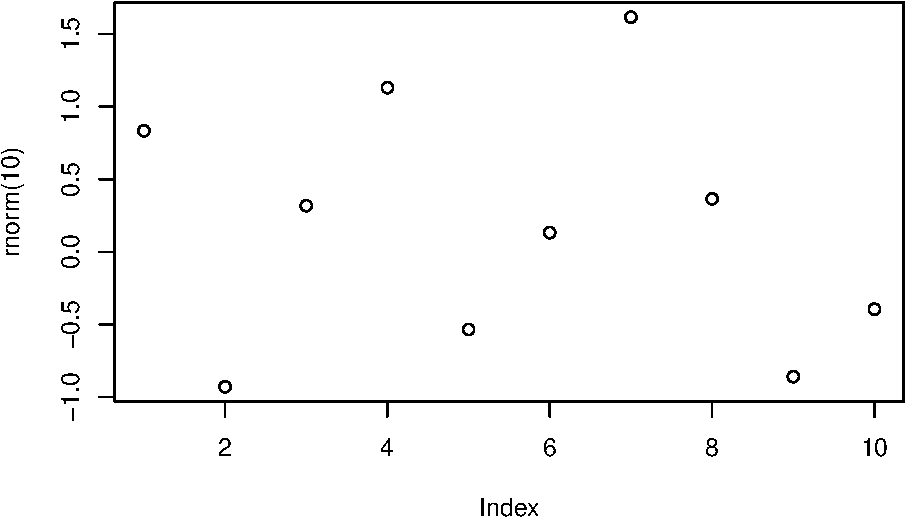
\includegraphics{../figures/demo-plot-1.pdf}
\caption{\label{fig:demo-plot}A plot of random numbers}
\end{figure}

Figure \ref{fig:demo-plot} shows how we can have a caption and cross-reference for a plot

Here is an example of inline code 3.14 in the middle of a sentence.

\hypertarget{discussion}{%
\section{Discussion}\label{discussion}}

\hypertarget{conclusion}{%
\section{Conclusion}\label{conclusion}}

\hypertarget{acknowledgements}{%
\section{Acknowledgements}\label{acknowledgements}}

\newpage

\hypertarget{references}{%
\section{References}\label{references}}

\hypertarget{refs}{}
\leavevmode\hypertarget{ref-Marwick2017}{}%
Marwick, B. 2017. Computational reproducibility in archaeological research: Basic principles and a case study of their implementation. Journal of Archaeological Method and Theory 24:424--450.

\newpage

\hypertarget{colophon}{%
\subsubsection{Colophon}\label{colophon}}

This report was generated on 2020-09-01 10:46:48 using the following computational environment and dependencies:

\begin{verbatim}
#> - Session info ---------------------------------------------------------------
#>  setting  value                       
#>  version  R version 4.0.2 (2020-06-22)
#>  os       macOS Catalina 10.15.6      
#>  system   x86_64, darwin17.0          
#>  ui       X11                         
#>  language (EN)                        
#>  collate  en_US.UTF-8                 
#>  ctype    en_US.UTF-8                 
#>  tz       America/Denver              
#>  date     2020-09-01                  
#> 
#> - Packages -------------------------------------------------------------------
#>  package     * version date       lib source        
#>  assertthat    0.2.1   2019-03-21 [1] CRAN (R 4.0.2)
#>  backports     1.1.9   2020-08-24 [1] CRAN (R 4.0.2)
#>  bookdown      0.20    2020-06-23 [1] CRAN (R 4.0.2)
#>  callr         3.4.3   2020-03-28 [1] CRAN (R 4.0.2)
#>  cli           2.0.2   2020-02-28 [1] CRAN (R 4.0.2)
#>  crayon        1.3.4   2017-09-16 [1] CRAN (R 4.0.2)
#>  desc          1.2.0   2018-05-01 [1] CRAN (R 4.0.2)
#>  devtools      2.3.1   2020-07-21 [1] CRAN (R 4.0.2)
#>  digest        0.6.25  2020-02-23 [1] CRAN (R 4.0.2)
#>  ellipsis      0.3.1   2020-05-15 [1] CRAN (R 4.0.2)
#>  evaluate      0.14    2019-05-28 [1] CRAN (R 4.0.1)
#>  fansi         0.4.1   2020-01-08 [1] CRAN (R 4.0.2)
#>  fs            1.5.0   2020-07-31 [1] CRAN (R 4.0.2)
#>  glue          1.4.2   2020-08-27 [1] CRAN (R 4.0.2)
#>  highr         0.8     2019-03-20 [1] CRAN (R 4.0.2)
#>  htmltools     0.5.0   2020-06-16 [1] CRAN (R 4.0.2)
#>  knitr         1.29    2020-06-23 [1] CRAN (R 4.0.2)
#>  magrittr      1.5     2014-11-22 [1] CRAN (R 4.0.2)
#>  memoise       1.1.0   2017-04-21 [1] CRAN (R 4.0.2)
#>  pkgbuild      1.1.0   2020-07-13 [1] CRAN (R 4.0.2)
#>  pkgload       1.1.0   2020-05-29 [1] CRAN (R 4.0.2)
#>  prettyunits   1.1.1   2020-01-24 [1] CRAN (R 4.0.2)
#>  processx      3.4.3   2020-07-05 [1] CRAN (R 4.0.2)
#>  ps            1.3.4   2020-08-11 [1] CRAN (R 4.0.2)
#>  R6            2.4.1   2019-11-12 [1] CRAN (R 4.0.2)
#>  remotes       2.2.0   2020-07-21 [1] CRAN (R 4.0.2)
#>  rlang         0.4.7   2020-07-09 [1] CRAN (R 4.0.2)
#>  rmarkdown     2.3     2020-06-18 [1] CRAN (R 4.0.2)
#>  rprojroot     1.3-2   2018-01-03 [1] CRAN (R 4.0.2)
#>  sessioninfo   1.1.1   2018-11-05 [1] CRAN (R 4.0.2)
#>  stringi       1.4.6   2020-02-17 [1] CRAN (R 4.0.2)
#>  stringr       1.4.0   2019-02-10 [1] CRAN (R 4.0.2)
#>  testthat      2.3.2   2020-03-02 [1] CRAN (R 4.0.2)
#>  usethis       1.6.1   2020-04-29 [1] CRAN (R 4.0.2)
#>  withr         2.2.0   2020-04-20 [1] CRAN (R 4.0.2)
#>  xfun          0.16    2020-07-24 [1] CRAN (R 4.0.2)
#>  yaml          2.2.1   2020-02-01 [1] CRAN (R 4.0.2)
#> 
#> [1] /Library/Frameworks/R.framework/Versions/4.0/Resources/library
\end{verbatim}

The current Git commit details are:

\end{document}
